\documentclass[11pt]{article}
\usepackage[margin=1in]{geometry}
\usepackage{amsmath,amssymb,amsthm,mathtools}
\usepackage{booktabs}
\usepackage{enumitem}
\usepackage{xcolor}
\usepackage{tikz}
\usepackage{tikz-cd}
\usetikzlibrary{arrows.meta,positioning,calc,fit,backgrounds,decorations.pathreplacing,shapes.geometric}
\definecolor{accent}{RGB}{196,78,30}
\definecolor{accentB}{RGB}{38,104,176}
\colorlet{blockfill}{accentB!7}
\colorlet{blockline}{accentB!45}
\colorlet{coarsefill}{accent!10}
\usepackage[hidelinks]{hyperref}
\usepackage[capitalise,noabbrev]{cleveref}

\newtheorem{theorem}{Theorem}[section]
\newtheorem{proposition}[theorem]{Proposition}
\newtheorem{lemma}[theorem]{Lemma}
\newtheorem{corollary}[theorem]{Corollary}
\theoremstyle{definition}
\newtheorem{definition}[theorem]{Definition}
\newtheorem{example}[theorem]{Example}
\theoremstyle{remark}
\newtheorem{remark}[theorem]{Remark}

\newcommand{\R}{\mathbb{R}}
\newcommand{\Lq}{\mathbb{L}}           % Lawvere quantale
\newcommand{\eps}{\varepsilon}
\newcommand{\dd}{d}
\newcommand{\Wm}{W^{\mathrm{must}}}
\newcommand{\Vm}{V^{\mathrm{must}}}
\newcommand{\tgt}{\star}

\title{Path Lifting for Hierarchical Planning:\\
Cost-Enriched Path Categories, Abstractions, and Sheaves on Covers}
\author{Draft --- CellularSheaves.jl working paper}
\date{\today}

\begin{document}
\maketitle

\begin{abstract}
We give a categorical account of hierarchical planning for deterministic, finite
control models such as the double integrator on a lattice. Three layers fit
together.
\begin{itemize}[nosep]
\item \emph{Dynamics.} The state graph generates a category of paths. Optimal
  costs enrich it in Lawvere's quantale of nonnegative reals, so the cost-to-go is
  a hom-object into a target and its subsolutions are exactly the presheaves.
\item \emph{Abstractions.} An abstraction is a map of cost graphs. Pulling back
  along it is sound for every abstraction: the coarse cost-to-go is always a lower
  bound.
\item \emph{Decompositions.} Covers of the state space, and covers of a set of
  agents, carry cellular sheaves of lattices on their nerves. The restriction maps
  are pullbacks along maps of cost graphs.
\end{itemize}
Our main result is a \emph{path-lifting theorem}. It measures how tight an
abstraction is by its \emph{lifting defect}: how much more than a coarse arc's
cost a state of the arc's source block must pay to follow it.
\begin{itemize}[nosep]
\item Zero defect on every coarse arc is equivalent to exactness of the coarse
  bound, for every target that is a union of blocks.
\item In general, the quotient with defect-inflated arc costs gives an upper bound
  that is never worse than the classical pessimistic (``must'') abstraction.
\end{itemize}
Within the categorical Lyapunov theory of Ames, Moeller and Tabuada, the same
bounds are Lyapunov certificates. The path category is a setting for stability
whose norm is the optimal cost-to-go. The two sides of the sandwich are the two
class-$\mathcal K$ bounds of a Lyapunov morphism, and the defect-inflated
quotient certifies a layered controller.
Experiments on a double integrator with $2.8$ million lattice states and on
cooperative multi-agent planning show the theorem's message in practice. The
natural maps are loose exactly where dynamics and constraints obstruct path
lifting: inclusions, forgetting velocity, position blocks, level sets. The maps
that work are the ones that lift better: velocity modes, Reeb arcs of the other
agents' value functions, and summaries refined by their reachable futures.
\end{abstract}

\section{Introduction}

Hierarchical planners solve a small problem to guide a large one. Hierarchical
A$^*$ searches the abstract space for an admissible heuristic~\cite{holte1996}.
Symbolic control synthesizes a controller on an abstraction and refines
it~\cite{tabuada2009,reissig2017}. Multi-agent planners bound the joint cost from
pairs~\cite{li2019}. In each case two questions arise.
\begin{itemize}[nosep]
\item Is the abstraction \emph{sound}, giving a valid bound or a valid refinement?
\item Is it \emph{tight}?
\end{itemize}
Soundness has many proofs, one per construction. Tightness is usually measured
only empirically.

This paper organizes both questions around one categorical picture and one
theorem.

\paragraph{Dynamics are enrichment.}
A finite state graph generates its free category, whose morphisms are paths.
Attaching nonnegative costs to arcs and keeping, for each pair of states, the
cheapest path turns the hom-sets into hom-objects in Lawvere's quantale
$([0,\infty], \ge, +, 0)$~\cite{lawvere1973}. The result is a generalized
(asymmetric) metric space: the shortest-path quasi-metric. Adding a sink $\tgt$
for the target, the cost-to-go is the hom-object $V(x) = \dd(x,\tgt)$. Its
subsolutions are exactly the presheaves on this space (\cref{sec:enriched}).
Solving for $V$ is computing a closure. This can be done by iteration, which is
the harmonic flow of a Lawvere Laplacian~\cite{ghrist2025diffusion}, by label
setting (Dijkstra, A$^*$), or by sparse elimination.

\paragraph{Abstractions are maps.}
A surjection $\psi$ of states onto blocks induces a quotient cost graph. It is the
largest one for which $\psi$ does not increase any arc's cost. Pulling the
quotient's cost-to-go back along $\psi$ is a lower bound for every $\psi$
(\cref{sec:abstraction}). Soundness is therefore functorial and comes for free.

\paragraph{Decompositions are sheaves.}
A cover of the state space, or of a set of agents, has a nerve. Value functions on
the pieces, with restriction maps given by pullback, form a cellular sheaf of
complete lattices in the sense of Ghrist and Riess~\cite{ghrist2022}
(\cref{sec:sheaves}). The canonical choice of restriction map is the inclusion of
a piece into a larger one. Any other map of cost graphs is also allowed, and
remains sound.

\paragraph{Tightness is path lifting.}
Our main result (\cref{sec:lifting}) characterizes when an abstraction is exact.
It is exact exactly when every coarse arc can be followed, at no more than its
cost, from \emph{every} state of its source block. The \emph{lifting defect}
measures the failure, and it bounds the loss: inflating the coarse arc costs by
their defects gives an upper bound on the true cost-to-go. This is the
cost-enriched counterpart of path-lifting properties familiar from concurrency
(open maps~\cite{joyal1996}) and from partition refinement (stable
partitions~\cite{paige1987}). Here costs are kept, and a lift may take any number
of steps.

\paragraph{The finding.}
Effective hierarchical planning for double integrators with obstacles, and for
several agents that must avoid collisions, requires restriction and abstraction
maps other than the obvious ones (\cref{sec:experiments}). The theorem says why.
\begin{itemize}[nosep]
\item Forgetting velocity cannot lift a coarse move from a state that is moving
  the other way.
\item Position blocks and level sets of another agent's value function cannot lift
  across walls or through corridors.
\end{itemize}
The maps that work, velocity modes, Reeb arcs and future-refined summaries, are
those with smaller defects.

\paragraph{Contributions.}
\begin{enumerate}[nosep]
\item A dictionary between finite deterministic optimal control and Lawvere-enriched
  path categories. It covers presheaves as subsolutions, quotients as maps,
  elimination as restriction to full subcategories, and fibres as distributors
  (\cref{sec:enriched,sec:abstraction}).
\item The path-lifting theorem: a sandwich bound and an exactness criterion
  (\cref{thm:sandwich,thm:exact}), with locality and may/must corollaries.
\item Lyapunov certificates in the categorical Lyapunov theory of Ames, Moeller
  and Tabuada~\cite{ames2025clt1}. Supersolutions with greedy feedback are
  Lyapunov morphisms whose class-$\mathcal K$ gains are certified by lower bounds,
  and both quotients yield certificates (\cref{sec:lyapunov}).
\item Sheaves of lattices on nerves of covers, with pullbacks along arbitrary maps
  of cost graphs as restriction maps, and their use for multi-agent planning
  (\cref{sec:sheaves}).
\item An empirical study connecting the theorem to measured tightness on a
  double-integrator lattice and on multi-agent problems (\cref{sec:experiments}).
\end{enumerate}
All constructions are implemented in the Julia package
\texttt{CellularSheaves.jl} (modules \texttt{TropicalAbstraction} and
\texttt{TropicalCovers}). Every number we report is regenerated by a script in its
\texttt{docs/scripts} directory.

\section{Cost-enriched path categories}\label{sec:enriched}

\begin{definition}
A \emph{cost graph} $(X, W)$ is a finite set $X$ of states with arc costs
$W : X \times X \to [0,\infty]$. We write $W(x,y) = \infty$ when there is no arc
$x \to y$. The cost of a path $x_0 \to x_1 \to \dots \to x_k$ is
$\sum_i W(x_i, x_{i+1})$, and the empty path at $x$ costs $0$.
\end{definition}

The free category on the graph has the paths as morphisms. Path cost is additive
under concatenation, so it is a functor from this category to the monoid
$([0,\infty], +, 0)$. Keeping only the cheapest path between each pair of states
gives
\[
\dd(x,y) = \min\{\text{cost}(p) : p \text{ a path } x \to y\}, \qquad
\dd(x,x) = 0, \qquad \dd(x,z) \le \dd(x,y) + \dd(y,z).
\]
Lawvere observed that such a $\dd$ is precisely a category enriched in the
symmetric monoidal closed category $\Lq = ([0,\infty], \ge, +, 0)$. In this view
the identities are $\dd(x,x)=0$, the triangle inequality is composition, and the
internal hom is truncated subtraction. None of his results need symmetry,
finiteness or separation~\cite[\S1]{lawvere1973}. Enriched functors are the
\emph{non-expansive} maps, $\dd'(fx, fy) \le \dd(x,y)$. We call $(X,\dd)$ the
\emph{path category} of $(X,W)$. It is the largest $\Lq$-category structure on $X$
below $W$: any quasi-metric $\dd'$ with $\dd' \le W$ on arcs satisfies
$\dd' \le \dd$, by the triangle inequality along each path.

\paragraph{Targets as an object.}
A terminal cost $b : X \to [0,\infty]$ (with $b = 0$ on a target set $\Gamma$ and
$\infty$ elsewhere, for reach problems) becomes part of the graph. Adjoin a sink
$\tgt$ with arcs $x \to \tgt$ of cost $b(x)$ and no arcs out of $\tgt$. The
\emph{cost-to-go} is the hom-object
\[ V(x) = \dd(x, \tgt) = \min_{y}\big(\dd(x,y) + b(y)\big). \]
Paths that end at the target are the morphisms into $\tgt$. Taking costs,
each hom-set becomes the cost of its optimal path.

\begin{definition}
A \emph{subsolution} is a function $f : X \to [0,\infty]$ with $f \le b$ and
$f(x) \le W(x,y) + f(y)$ for every arc. A \emph{supersolution} satisfies
$\min\big(b(x), \min_y W(x,y) + f(y)\big) \le f(x)$ for every $x$.
\end{definition}

The supersolution condition says that from every state either stopping or some
move costs no more than $f$ predicts. It is the discrete control Lyapunov
inequality.

\begin{proposition}\label{prop:presheaf}
Extend $f$ by $f(\tgt) = 0$. Then $f$ is a subsolution if and only if
$f(x) \le \dd(x,y) + f(y)$ for all $x, y \in X \cup \{\tgt\}$. Equivalently,
$f$ is an $\Lq$-functor $(X \cup\{\tgt\})^{\mathrm{op}} \to \Lq$ (a presheaf),
where $\Lq$ carries its internal hom $[a, c] = \max(c - a, 0)$. The cost-to-go
$V = \dd(-,\tgt)$ is the greatest subsolution.
\end{proposition}
\begin{proof}
The arc conditions, including those into $\tgt$, sum along every path, which gives
the first equivalence. A functor $(X\cup\{\tgt\})^{\mathrm{op}} \to \Lq$ must
satisfy $\dd(x,y) \ge [f(y), f(x)] = \max(f(x) - f(y), 0)$ in the order of $\Lq$.
This is the same inequality. Taking $y = \tgt$ gives $f(x) \le \dd(x,\tgt) = V(x)$,
and $V$ is itself a subsolution by the triangle inequality.
\end{proof}

The subsolutions are the post-fixed points $f \le Bf$ of the monotone Bellman
operator $(Bf)(x) = \min\big(b(x), \min_y W(x,y) + f(y)\big)$ on the complete
lattice $[0,\infty]^X$. By Tarski's theorem~\cite{tarski1955} its fixed points form
a complete lattice, and $V$ is the greatest fixed point. With zero-cost cycles
there can be other fixed points, so we obtain upper bounds by constructing walks
(\cref{sec:lifting}) rather than from arbitrary supersolutions.

\paragraph{Three ways to compute $V$.}
\begin{enumerate}[nosep]
\item \emph{Iteration.} Iterating $f \mapsto f \wedge Bf$ from $b$ is Bellman's
  method~\cite{bellman1958}. Ghrist, Lopez, North and Riess introduce the
  \emph{Lawvere Laplacian} of a network sheaf valued in quantale-enriched
  categories, together with a weighting $W : V \times V \to Q$ that relaxes
  agreement along each edge in each direction (their Definition~3.2). For
  a crisp Laplacian, its suffix points are the $W$-fuzzy global sections
  (their Theorem~3.17)~\cite{ghrist2025diffusion}. In their shortest-path
  example (their \S4.2) the sheaf is constant with stalk the Lawvere reals (with
  the opposite order) and the graph is undirected with symmetric weights. The
  Laplacian is $(L_W x)_v = \min_{w \in N_v} W(v,w) + x_w$, and their harmonic
  flow $x \mapsto x \wedge L_W x$ is the iteration above. Their Definition~3.2
  allows $W(v,w) \ne W(w,v)$. With $W(v,w)$ the cost of the arc $v \to w$ (and
  $\infty$ when absent), the $W$-fuzzy sections are exactly the presheaves of
  \cref{prop:presheaf} without the target. The asymmetric reading is ours, and
  their paper is a preprint.
\item \emph{Label setting.} Dijkstra's algorithm~\cite{dijkstra1959} computes $V$
  by exploiting the order. A$^*$~\cite{hart1968} is Dijkstra's algorithm on the
  reduced costs $W(x,y) + h(y) - h(x)$ of a consistent heuristic $h$, the same
  reweighting Johnson used to remove negative arcs~\cite{johnson1977}.
\item \emph{Elimination.} $V$ is a column of the closure
  $W^* = I \oplus W \oplus W^{\otimes 2} \oplus \cdots$ in the min-plus semiring.
  Gaussian elimination in closed semirings computes it~\cite{carre1971,lehmann1977}.
\end{enumerate}

\begin{proposition}[elimination is restriction to a full subcategory]\label{prop:schur}
Split $X = S \sqcup I$ and write $W$ in blocks. Then
\[
(W^*)_{SS} = \big(W_{SS} \oplus W_{SI} \otimes W_{II}^* \otimes W_{IS}\big)^* .
\]
That is, the path category of the reduced graph on $S$ is the full subcategory of
$(X,\dd)$ on $S$.
\end{proposition}
\begin{proof}
A path between states of $S$ splits at its visits to $S$ into arcs inside $S$ and
excursions $S \to I \to \cdots \to I \to S$. The cheapest excursion from $s$ to $s'$
costs $(W_{SI} \otimes W_{II}^* \otimes W_{IS})(s,s')$. Minimizing over all such
decompositions gives the right-hand side.
\end{proof}

The same formula defines the star of a $2 \times 2$ block matrix over a Kleene
algebra~\cite{kozen1994}. Lehmann notes that it does not hold in every closed
semiring, only under additional identities due to Conway~\cite{lehmann1977}. The
path argument above suffices for nonnegative costs.

This is the min-plus counterpart of Kron reduction, the Schur complement of a
graph Laplacian onto boundary nodes, which is again a graph
Laplacian~\cite{dorfler2013}. It is also harmonic extension through the
eliminated interior: the reduced graph on a separator holds everything the
interior can contribute. The contrast with real sheaves is instructive. Hansen and
Ghrist show that Kron reduction of sheaf Laplacians is not possible in general;
their positive result needs vertex stalks of dimension at most one
(their \S4.2)~\cite{hansen2019}. Min-plus elimination, by contrast, always
returns a cost graph.

\section{Abstractions as maps of cost graphs}\label{sec:abstraction}

\begin{definition}
An \emph{abstraction} is a surjection $\psi : X \to Y$. Its fibres
$B = \psi^{-1}(B)$ are the \emph{blocks}. The \emph{optimistic quotient} is
\[
W_\psi(B, C) = \min_{x \in B,\, y \in C} W(x,y) \quad (B \ne C), \qquad
b_\psi(B) = \min_{x \in B} b(x),
\]
and arcs inside a block are contracted. The \emph{pessimistic quotient} is
\[
\Wm(B,C) = \max_{x \in B} \min_{y \in C} W(x,y) \quad (B \ne C), \qquad
b^{\mathrm{must}}(B) = \max_{x \in B} b(x).
\]
We write $V_\psi$ and $\Vm$ for their cost-to-go functions on $Y$.
\end{definition}

The two quotients are the ``may'' and ``must'' transitions of modal transition
systems~\cite{larsen1988}.

\begin{proposition}\label{prop:quotient-map}
$W_\psi$ is the greatest arc weighting on $Y$ such that
$W_\psi(\psi x, \psi y) \le W(x,y)$ for every arc between different blocks. Hence
$\psi$ is non-expansive from $(X,\dd)$ to the path category $(Y,\dd_\psi)$, and
$b_\psi(\psi x) \le b(x)$.
\end{proposition}
\begin{proof}
The first claim is the definition of a minimum. An arc inside a block maps to an
identity of cost $0 \le W(x,y)$. Summing along paths gives
$\dd_\psi(\psi x, \psi y) \le \dd(x,y)$.
\end{proof}

\paragraph{Pullback and pushforward.}
Let $E g = g \circ \psi$ and $(Pf)(B) = \min_{x \in B} f(x)$. Then
$Eg \le f \iff g \le Pf$, so $E \dashv P$ is a Galois connection with $PE = I$
and $EP \le I$. No normalization is needed, because $\min$ is idempotent. In the
min-plus semiring the optimistic quotient is the ``Galerkin'' product
$P \otimes W \otimes E$ with the diagonal contracted. This is the same formula as
the coarse operator of an aggregation multigrid method, but it is used to bound
rather than to correct. The max-plus finite element method of Akian, Gaubert and
Lakhoua projects Bellman operators with residuated projections of exactly this
kind~\cite{akian2008,cohen2004}.

\begin{proposition}[soundness]\label{prop:lower}
$E V_\psi = V_\psi \circ \psi \le V$.
\end{proposition}
\begin{proof}
$V_\psi$ is a presheaf on $Y \cup \{\tgt\}$. Precomposition with the non-expansive
map $\psi$ (extended by $\tgt \mapsto \tgt$) gives a presheaf on
$X \cup \{\tgt\}$, that is, a subsolution by \cref{prop:presheaf}. $V$ is the
greatest subsolution.
\end{proof}

The proof uses nothing about $\psi$ except that it is a map. Any composite of
abstractions, restrictions to unions of blocks, products of abstractions, or
changes of gauge is therefore sound. Abstraction distances as admissible
heuristics are the basis of Hierarchical A$^*$~\cite{holte1996} and of pattern
databases~\cite{culberson1998}.

\paragraph{Fibres as distributors.}
For blocks $B, C$ let $D_{BC} = \dd|_{B \times C}$ be the matrix of fine distances
from $B$ to $C$. Each $(B, D_{BB})$ is an $\Lq$-category, and each $D_{BC}$ is an
$\Lq$-distributor (profunctor) from $B$ to $C$. The triangle inequality gives
\[
D_{CE} \otimes D_{BC} \;\ge\; D_{BE}, \qquad D_{BB} \otimes D_{BC} = D_{BC},
\]
entrywise, in min-plus products, and $D_{BB}$ has zero diagonal. So the blocks
and the matrices $D_{BC}$ form a category enriched in the bicategory of
$\Lq$-valued matrices, with object set $Y$. Equivalently, by Bénabou's
observation as recorded by Street, they form a lax functor from the chaotic
category on $Y$ into that bicategory~\cite{street1983}. Regarding each fibre as
the $\Lq$-category $(B, D_{BB})$, each $D_{BC}$ is a distributor and the lax
functor is normal. For ordinary categories, Bénabou associates with any functor
$P : \mathcal X \to \mathcal I$ a normalized lax functor from
$\mathcal I^{\mathrm{op}}$ into distributors. Its value at an object is the fibre,
and its value at a morphism $\alpha$ is the set of morphisms over
$\alpha$~\cite{benabou2000}. Our statement is a cost-enriched analogue over the
chaotic category, proved directly above. In this picture the ``stalk over a coarse
cell'' is a fibre and the ``transfer between stalks'' is a distributor. Neither is
a restriction map of a cellular sheaf. Arcs between fibres are directed, and
nothing here needs an orientation.

\begin{remark}[gauge]
For a potential $\varphi$ that is consistent ($\varphi(x) \le W(x,y) + \varphi(y)$),
the reduced costs $W^\varphi(x,y) = W(x,y) + \varphi(y) - \varphi(x)$ are
nonnegative. The fine problem changes only by $V^\varphi = V - \varphi$. The quotient
does change, because a minimum over a block does not commute with adding
different amounts to different states. The bound $\varphi + E V^\varphi_\psi$ is
again sound by \cref{prop:lower}. This is potential-based shaping~\cite{ng1999}
applied to the abstraction rather than to the search.
\end{remark}

\section{The path-lifting theorem}\label{sec:lifting}

\begin{definition}\label{def:defect}
For an arc $B \to C$ of $W_\psi$ ($B \ne C$, $W_\psi(B,C) < \infty$) and for the
terminal arc of $B$ ($b_\psi(B) < \infty$), the \emph{lifting defects} are
\[
\eps_\psi(B,C) = \max_{x \in B}\big(\dd(x,C) - W_\psi(B,C)\big)^+, \qquad
\eps_\psi(B,\tgt) = \max_{x \in B}\big(V(x) - b_\psi(B)\big)^+,
\]
where $\dd(x,C) = \min_{y\in C}\dd(x,y)$ and $(t)^+ = \max(t,0)$. The arc
\emph{lifts} if its defect is $0$: every state of $B$ can reach $C$ (respectively,
the target) at no more than the coarse arc's cost. Let $V_\psi^{+\eps}$ be the
cost-to-go of the quotient with arc costs $W_\psi + \eps_\psi$ and terminal costs
$b_\psi + \eps_\psi(\cdot,\tgt)$.
\end{definition}

In the distributor picture, $\eps_\psi(B,C)$ is the worst row minimum of $D_{BC}$
minus the coarse arc cost. An arc lifts when no row of the distributor is worse
than its cheapest entry. A lift may use any number of fine steps, including steps
inside $B$ or through other blocks.

\begin{theorem}[sandwich]\label{thm:sandwich}
For every $x \in X$,
\[
V_\psi(\psi x) \;\le\; V(x) \;\le\; V_\psi^{+\eps}(\psi x) \;\le\; \Vm(\psi x).
\]
\end{theorem}
\begin{proof}
The first inequality is \cref{prop:lower}.

For the second, let $B_0 = \psi x \to B_1 \to \dots \to B_k \to \tgt$ be an optimal
walk for $W_\psi + \eps_\psi$ (if none exists the bound is $\infty$). Set
$x_0 = x$. Given $x_i \in B_i$, the definition of the defect gives
$\dd(x_i, B_{i+1}) \le W_\psi(B_i,B_{i+1}) + \eps_\psi(B_i,B_{i+1})$. Pick
$x_{i+1} \in B_{i+1}$ attaining $\dd(x_i, B_{i+1})$. At the end,
$V(x_k) \le b_\psi(B_k) + \eps_\psi(B_k,\tgt)$. By the triangle inequality,
$V(x) \le \sum_i \dd(x_i,x_{i+1}) + V(x_k) \le V_\psi^{+\eps}(B_0)$.

For the third, let $B \to C$ be an arc of $\Wm$. Then $W_\psi(B,C)$ is finite, and
every $x \in B$ has an arc into $C$, so
$\dd(x,C) \le \min_{y \in C} W(x,y) \le \Wm(B,C)$. Hence
$W_\psi + \eps_\psi \le \Wm$ on the arcs of $\Wm$. Likewise
$V(x) \le b(x) \le b^{\mathrm{must}}(B)$ gives
$b_\psi + \eps_\psi(\cdot,\tgt) \le b^{\mathrm{must}}$. Every walk of the
pessimistic quotient is a walk of the inflated one and costs no less there.
\end{proof}

\begin{theorem}[exactness is lifting]\label{thm:exact}
The following are equivalent:
\begin{enumerate}[label=(\roman*),nosep]
\item $V_\psi \circ \psi = V$ for every target $\Gamma$ that is a union of blocks
  ($b = 0$ on $\Gamma$, $\infty$ elsewhere);
\item $\eps_\psi(B,C) = 0$ for every arc $B \to C$ of $W_\psi$ between distinct
  blocks.
\end{enumerate}
When they hold, $V_\psi \circ \psi = V$ for every terminal cost constant on blocks.
\end{theorem}
\begin{proof}
(i)$\Rightarrow$(ii). Take $\Gamma = C$. For $x \in B$,
$\dd(x,C) = V(x) = V_\psi(B) \le W_\psi(B,C)$.

(ii)$\Rightarrow$(i). Let $b$ be constant on blocks. Then $b_\psi(\psi x) = b(x)$,
so $V(x) \le b(x) = b_\psi(\psi x)$ and the terminal defects vanish. All defects
are $0$, so $V_\psi^{+\eps} = V_\psi$, and \cref{thm:sandwich} gives equality.
\end{proof}

\begin{corollary}[quantitative form]\label{cor:quant}
Let $\eps_{\max}$ be the largest defect, and let $\kappa(B)$ be the fewest arcs,
the terminal arc included, on an optimal walk of $W_\psi$ from $B$. Then
$V(x) \le V_\psi(\psi x) + \kappa(\psi x)\,\eps_{\max}$.
\end{corollary}
\begin{proof}
Lift that walk as in the proof of \cref{thm:sandwich}.
\end{proof}

\begin{corollary}[may/must gap]\label{cor:gap}
On every arc of $\Wm$, $\eps_\psi(B,C) \le \Wm(B,C) - W_\psi(B,C)$. The gap between
the two quotients bounds the defect, and with it the loss of the optimistic bound.
\end{corollary}

\begin{figure}[t]
\centering
% Optimistic quotient, pessimistic quotient, lifting defect and the sandwich.
% Fine graph: x1 -> y1 (1), x2 -> y2 (3), x2 -> x1 (1). Target: block C.
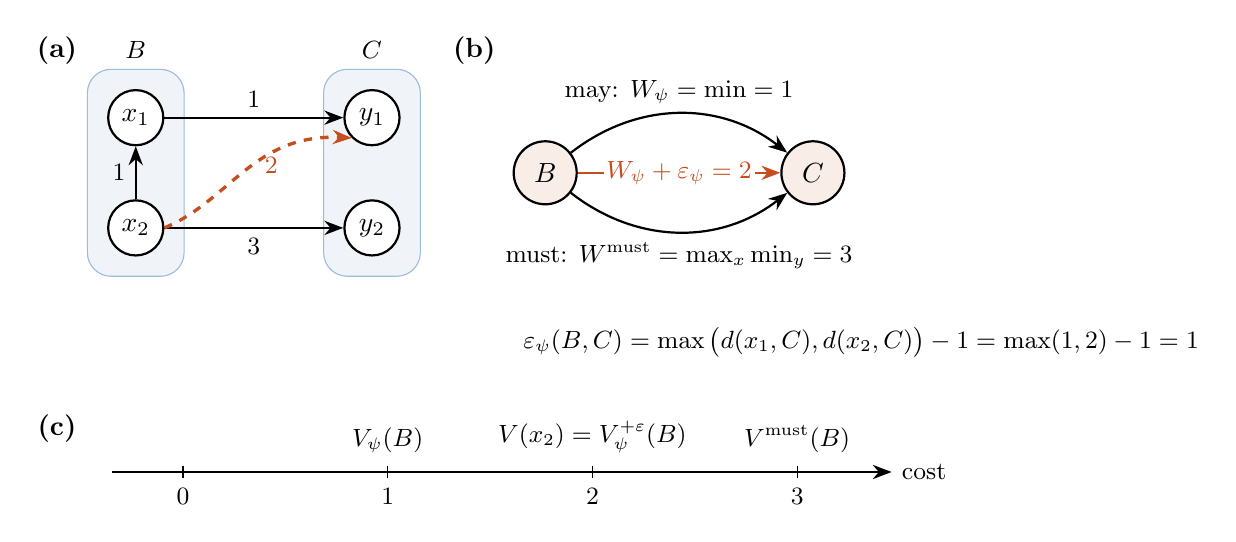
\begin{tikzpicture}[
    st/.style={circle, draw, thick, minimum size=7mm, inner sep=0pt, fill=white},
    arc/.style={-{Stealth[length=2.4mm]}, thick},
    lift/.style={-{Stealth[length=2.4mm]}, very thick, accent, dashed},
    blk/.style={rounded corners=3mm, draw=blockline, fill=blockfill, inner sep=2.5mm},
    cs/.style={circle, draw, thick, minimum size=8mm, inner sep=0pt, fill=coarsefill},
    lab/.style={font=\small},
  ]
  % ------------------------------------------------------------ fine graph
  \node[st] (x1) at (0,1.2) {$x_1$};
  \node[st] (x2) at (0,-0.2) {$x_2$};
  \node[st] (y1) at (3,1.2) {$y_1$};
  \node[st] (y2) at (3,-0.2) {$y_2$};
  \begin{scope}[on background layer]
    \node[blk, fit=(x1)(x2), label={[lab]above:$B$}] {};
    \node[blk, fit=(y1)(y2), label={[lab]above:$C$}] {};
  \end{scope}
  \draw[arc] (x1) -- node[lab, above] {$1$} (y1);
  \draw[arc] (x2) -- node[lab, below] {$3$} (y2);
  \draw[arc] (x2) -- node[lab, left] {$1$} (x1);
  \draw[lift] (x2.east) .. controls (1.2,0.15) and (1.5,1.0) .. node[lab, right, pos=0.55] {$2$} (y1.south west);
  \node[font=\bfseries] at (-1.0,2.05) {(a)};

  % ------------------------------------------------------------ the three coarse arcs
  \begin{scope}[xshift=5.2cm]
    \node[cs] (B) at (0,0.5) {$B$};
    \node[cs] (C) at (3.4,0.5) {$C$};
    \draw[arc] (B) to[bend left=38] node[lab, above] {may: $W_\psi = \min = 1$} (C);
    \draw[arc, accent] (B) -- node[lab, fill=white, inner sep=1pt] {$W_\psi + \eps_\psi = 2$} (C);
    \draw[arc] (B) to[bend right=38] node[lab, below] {must: $\Wm = \max_x \min_y = 3$} (C);
    \node[lab, align=left, anchor=west] at (-0.4,-1.65)
      {$\eps_\psi(B,C) = \max\big(\dd(x_1,C), \dd(x_2,C)\big) - 1 = \max(1,2) - 1 = 1$};
    \node[font=\bfseries] at (-0.9,2.05) {(b)};
  \end{scope}

  % ------------------------------------------------------------ sandwich at x2, target C
  \begin{scope}[yshift=-3.3cm]
    \draw[-{Stealth[length=2.4mm]}, thick] (-0.3,0) -- (9.6,0) node[right, lab] {cost};
    \foreach \t in {0,1,2,3} { \draw (\t*2.6+0.6,0.08) -- ++(0,-0.16) node[below, lab] {$\t$}; }
    \node[lab, above] (l) at (1*2.6+0.6,0.12) {$V_\psi(B)$};
    \node[lab, above, align=center] at (2*2.6+0.6,0.12) {$V(x_2) = V^{+\eps}_\psi(B)$};
    \node[lab, above] at (3*2.6+0.6,0.12) {$\Vm(B)$};
    \node[font=\bfseries] at (-1.0,0.55) {(c)};
  \end{scope}
\end{tikzpicture}

\caption{The two quotients and the defect. (a) The cheapest arc into $C$ leaves
$x_1$ and costs $1$. The arc out of $x_2$ costs $3$, but $x_2$ reaches $C$ for $2$
through $x_1$ (dashed). (b) The optimistic arc $B \to C$ costs $1$ and the
pessimistic arc costs $3$. The defect is $1$, so the defect-inflated arc costs
$2$, as in \cref{cor:gap}. (c) The sandwich of \cref{thm:sandwich} at $x_2$ for
the target $C$.}
\label{fig:quotients}
\end{figure}

\begin{proposition}[locality]\label{prop:local}
\Cref{thm:sandwich} remains true when $\dd(x,C)$ and $V$ in \cref{def:defect} are
replaced by any upper bounds. In particular, distances computed in the subgraph
on $B \cup C$ alone give computable upper bounds on the defects.
\end{proposition}
\begin{proof}
The proof of \cref{thm:sandwich} uses only the inequalities
$\dd(x_i,B_{i+1}) \le W_\psi + \eps$ and $V(x_k) \le b_\psi + \eps$.
\end{proof}

\begin{example}[gauge and defect]\label{ex:line}
Take the line $1 \to 2 \to 3 \to 4$ with unit costs, target $4$, and blocks
$A = \{1,2\}$, $B = \{3,4\}$. The arc $A \to B$ costs $1$ (the arc $2 \to 3$), but
$\dd(1, B) = 2$, so $\eps_\psi(A,B) = 1$. The bound at state $1$ is $1$ against a
true cost of $3$. In the gauge $\varphi = V = (3,2,1,0)$ every arc costs $0$, the
defect vanishes, and the bound $\varphi + E V^\varphi_\psi$ is exact. The gauge
moves information out of arc costs, which the minimum over a block destroys, into
the potential, which is added back state by state.
\end{example}

\begin{figure}[t]
\centering
% Example (gauge and defect): the line 1 -> 2 -> 3 -> 4, blocks A = {1,2}, B = {3,4}.
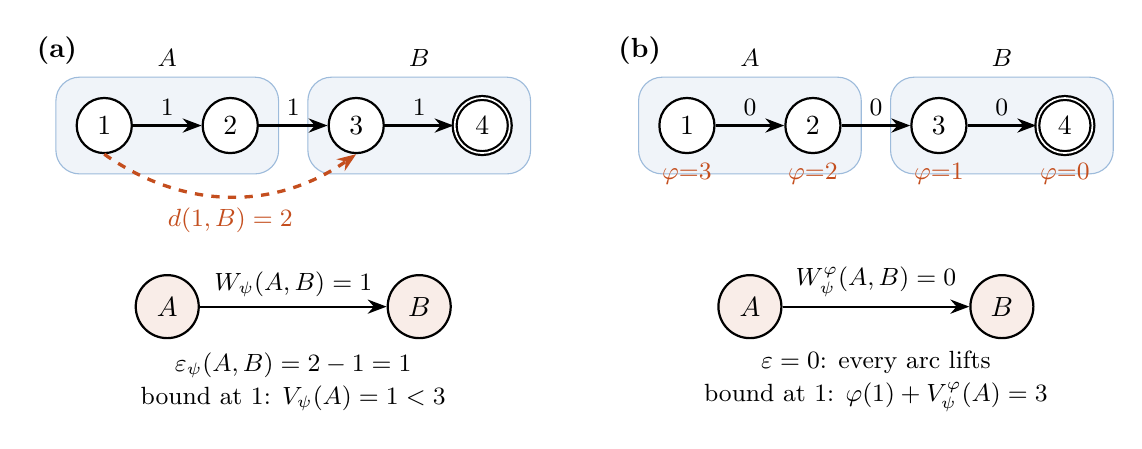
\begin{tikzpicture}[
    st/.style={circle, draw, thick, minimum size=7mm, inner sep=0pt, fill=white},
    tg/.style={st, double},
    arc/.style={-{Stealth[length=2.4mm]}, thick},
    lift/.style={-{Stealth[length=2.4mm]}, very thick, accent, dashed},
    blk/.style={rounded corners=3mm, draw=blockline, fill=blockfill, inner sep=2.5mm},
    cs/.style={circle, draw, thick, minimum size=8mm, inner sep=0pt, fill=coarsefill},
    lab/.style={font=\small},
  ]
  % ------------------------------------------------------------ (a) plain costs
  \begin{scope}
    \node[st] (a1) at (0,0) {$1$};
    \node[st] (a2) at (1.6,0) {$2$};
    \node[st] (a3) at (3.2,0) {$3$};
    \node[tg] (a4) at (4.8,0) {$4$};
    \begin{scope}[on background layer]
      \node[blk, fit=(a1)(a2), label={[lab]above:$A$}] {};
      \node[blk, fit=(a3)(a4), label={[lab]above:$B$}] {};
    \end{scope}
    \draw[arc] (a1) -- node[lab, above] {$1$} (a2);
    \draw[arc] (a2) -- node[lab, above] {$1$} (a3);
    \draw[arc] (a3) -- node[lab, above] {$1$} (a4);
    \draw[lift] (a1.south) to[out=-35, in=-145] node[lab, below] {$\dd(1,B) = 2$} (a3.south);
    % coarse
    \node[cs] (A) at (0.8,-2.3) {$A$};
    \node[cs] (B) at (4.0,-2.3) {$B$};
    \draw[arc] (A) -- node[lab, above] {$W_\psi(A,B) = 1$} (B);
    \node[lab, align=center] at (2.4,-3.25) {$\eps_\psi(A,B) = 2 - 1 = 1$\\[1pt] bound at $1$: $V_\psi(A) = 1 < 3$};
    \node[font=\bfseries] at (-0.6,0.95) {(a)};
  \end{scope}
  % ------------------------------------------------------------ (b) gauge phi = V
  \begin{scope}[xshift=7.4cm]
    \node[st] (b1) at (0,0) {$1$};
    \node[st] (b2) at (1.6,0) {$2$};
    \node[st] (b3) at (3.2,0) {$3$};
    \node[tg] (b4) at (4.8,0) {$4$};
    \begin{scope}[on background layer]
      \node[blk, fit=(b1)(b2), label={[lab]above:$A$}] {};
      \node[blk, fit=(b3)(b4), label={[lab]above:$B$}] {};
    \end{scope}
    \draw[arc] (b1) -- node[lab, above] {$0$} (b2);
    \draw[arc] (b2) -- node[lab, above] {$0$} (b3);
    \draw[arc] (b3) -- node[lab, above] {$0$} (b4);
    \foreach \i/\v in {1/3, 2/2, 3/1, 4/0} {
      \node[lab, text=accent] at ($(b\i) + (0,-0.62)$) {$\varphi{=}\v$};
    }
    \node[cs] (A2) at (0.8,-2.3) {$A$};
    \node[cs] (B2) at (4.0,-2.3) {$B$};
    \draw[arc] (A2) -- node[lab, above] {$W^\varphi_\psi(A,B) = 0$} (B2);
    \node[lab, align=center] at (2.4,-3.25) {$\eps = 0$: every arc lifts\\[1pt] bound at $1$: $\varphi(1) + V^\varphi_\psi(A) = 3$};
    \node[font=\bfseries] at (-0.6,0.95) {(b)};
  \end{scope}
\end{tikzpicture}

\caption{The line of \cref{ex:line}. (a) The coarse arc $A \to B$ costs $1$,
realised by $2 \to 3$. From state $1$, reaching $B$ costs $2$ (dashed), so the arc
has defect $1$, and the bound at $1$ is $1$ against a true cost of $3$. (b) In the
gauge $\varphi = V$ every arc costs $0$ and every arc lifts, so the bound
$\varphi + E V^\varphi_\psi$ is exact.}
\label{fig:line}
\end{figure}

\paragraph{Boolean special cases.}
Restrict attention to a set of arcs of equal cost, for example the zero-cost arcs
in the gauge of a relaxation. Then an arc lifts in one step from every state of
its block exactly when $\psi$ is \emph{locally surjective} on those arcs: every
state of a block reaches the same blocks. This is Paige and Tarjan's stability: a block $B$ is stable with respect to $S$
if $B \subseteq E^{-1}(S)$ or $B \cap E^{-1}(S) = \emptyset$. The coarsest stable
refinement of a partition is their relational coarsest
partition~\cite{paige1987}. For labelled transition systems, the morphisms that
lift every transition from every reachable state are the ``zig-zag'' morphisms.
Joyal, Nielsen and Winskel identify these as the open maps for the category of
branches, and define bisimilarity by spans of open maps~\cite{joyal1996}. \Cref{def:defect} relaxes these conditions in two
ways: a lift may take several steps, and it may cost more, with the excess
recorded as the defect. The relaxation matters. On a grid, the stable refinement of
a summary for zero-delay moves splits it down to single cells
(\cref{sec:experiments}), so exact lifting gives no compression. The useful
abstractions have small but nonzero defects.

\paragraph{Numerical check.}
The script \texttt{docs/scripts/path\_lifting\_check.jl} checks every statement of
this section on 3000 random cost graphs with random partitions and terminal costs
(1026 of them with zero defect), with no failures.

\section{Lyapunov certificates}\label{sec:lyapunov}

The sandwich of \cref{thm:sandwich} brackets the cost-to-go. This section shows
that the same brackets are Lyapunov certificates for closed loops, in the sense of
the categorical Lyapunov theory of Ames, Moeller and
Tabuada~\cite{ames2025clt1}. In their framework a Lyapunov function is a
\emph{Lyapunov morphism} $V : E \to R$ into a posetal ``stable object'' $R$.
\begin{itemize}[nosep]
\item Positive definiteness and decrease are lax commuting diagrams.
\item The existence of a Lyapunov morphism implies stability of an equilibrium
  (their Theorem~1, the categorical Lyapunov theorem).
\end{itemize}
They instantiate the framework for discrete-time systems and for Lawvere metric
spaces (their \S4.2 and \S5.2). The cost-enriched path categories of
\cref{sec:enriched} are an instance of both.

\paragraph{A setting for stability whose norm is the cost-to-go.}
Collapse the target set $\Gamma$ into the sink $\tgt$, and assume every arc out of
a state of $X$ costs at least $c > 0$. Let $E$ be the set of states with
$V < \infty$, together with $\tgt$. Following their Definition~4, take:
\begin{itemize}[nosep]
\item the category $\mathbf{Set}$ (S0) and the space $E$ (S1);
\item time $(\mathbb Z_{\ge 0}, +, 0)$ (S2);
\item the stable object $R = [0,\infty]$ with its usual order and point $0$ (S3);
\item the distance $\dd$, the path quasi-metric of \cref{sec:enriched} (S4).
\end{itemize}
Axiom S4 asks for $\dd \ge 0$ and $\dd(x,y) = 0$ only when $x = y$. The latter
holds because arc costs are positive; symmetry is not required. Their norm
relative to the equilibrium $\tgt$ (their Definition~5) is
\[ \|x\|_{\tgt} = \dd(x, \tgt) = V(x). \]
\emph{In this setting the norm is the optimal cost-to-go.}

A feedback $\pi : E \to E$ with $\pi(\tgt) = \tgt$, taking each state along one
of its arcs, gives the discrete-time flow $\phi(k, x) = \pi^k(x)$ with equilibrium
$\tgt$ (their \S4.2). A \emph{Lyapunov morphism} (their Definition~13) is a map
$f : E \to [0,\infty]$ with two properties:
\begin{itemize}[nosep]
\item \emph{positive definite}: there are class-$\mathcal K$ maps
  $\underline\alpha, \overline\alpha$ (order-preserving bijections of $[0,\infty]$
  fixing $0$) with
  $\underline\alpha(\|x\|_\tgt) \le f(x) \le \overline\alpha(\|x\|_\tgt)$;
\item \emph{decrescent}: $f(\pi(x)) \le f(x)$.
\end{itemize}
Their Theorem~1 then gives stability: $\|\pi^k(x)\|_\tgt \le
\underline\alpha^{-1}\overline\alpha(\|x\|_\tgt)$.

\begin{proposition}[supersolutions are Lyapunov morphisms]\label{prop:clf}
Let $f$ be a supersolution with $f(\tgt) = 0$, let $E_f = \{f < \infty\}$, and let
$\pi$ be a greedy feedback: $W(x,\pi x) + f(\pi x) \le f(x)$ for $x \in E_f
\setminus \{\tgt\}$. Then:
\begin{enumerate}[label=(\roman*),nosep]
\item $\pi$ maps $E_f$ into itself, and $f(\pi x) \le f(x) - c$ off $\tgt$;
\item $V \le f$ on $E_f$, so $\underline\alpha = \mathrm{id}$ is a lower class-$\mathcal K$ bound;
\item $\overline\alpha(t) = \kappa_f\, t$ with
  $\kappa_f = \max_{x \in E_f \setminus\{\tgt\}} f(x)/V(x)$ is an upper
  class-$\mathcal K$ bound;
\item hence $f$ is a Lyapunov morphism for $\pi$ on $E_f$. The closed loop reaches
  $\tgt$ from $x$ within $f(x)/c$ steps, at total cost at most
  $f(x) \le \kappa_f V(x)$.
\end{enumerate}
\end{proposition}
\begin{proof}
(i) is the greedy inequality together with $W \ge c$. By (i), $f$ decreases by at
least $c$ per step, so the closed loop from $x$ reaches $\tgt$ within $f(x)/c$
steps. Summing the greedy inequality along the way, its cost is at most $f(x)$.
Since $V(x)$ is the cheapest cost, $V(x) \le f(x)$, which is (ii). For (iii),
$E_f$ is finite and $V > 0$ off $\tgt$, so $\kappa_f < \infty$, and $t \mapsto
\kappa_f t$ is an order-preserving bijection of $[0,\infty]$ fixing $0$. (iv)
combines (i)--(iii) with their Definition~13.
\end{proof}

Finite-time reach is our addition. Their Theorem~1 concludes stability, while the
strict decrease in (i) gives reachability.

The useful reading is the following. The two lax triangles of positive
definiteness are the two sides of our sandwich. The upper gain $\kappa_f$ involves
the unknown $V$, but any subsolution $L \le V$ bounds it:
\[
\begin{tikzcd}[column sep=large]
& E \arrow[dl, "L"'] \arrow[d, "\|\cdot\|_\tgt = V" description] \arrow[dr, "f"] & \\
{[0,\infty]} \arrow[r, phantom, "\le"] & {[0,\infty]} \arrow[r, phantom, "\le"] & {[0,\infty]}
\end{tikzcd}
\qquad\qquad
f \le \kappa\, L \le \kappa\, V, \quad \kappa = \max_{x \ne \tgt} \frac{f(x)}{L(x)}
\quad (L > 0 \text{ off } \tgt).
\]
So a lower bound from an optimistic abstraction ($L = V_\psi \circ \psi$,
\cref{prop:lower}) certifies the class-$\mathcal K$ gain, and with it the
suboptimality of the closed loop, without computing $V$. This is the
``guaranteed bound'' of \cref{sec:experiments}.

\begin{theorem}[Lyapunov certificates from abstractions]\label{thm:lyap-abstraction}
Let $\psi$ be an abstraction and let the target be a union of blocks, so that
$V_\psi \circ \psi > 0$ off the target.
\begin{enumerate}[label=(\alph*),nosep]
\item \emph{Pessimistic.} $\Vm \circ \psi$ is a supersolution. With its greedy
  feedback, it is a Lyapunov morphism on $\{\Vm \circ \psi < \infty\}$, with gain
  at most $\max \Vm\circ\psi / V_\psi \circ \psi$.
\item \emph{Lifted.} Define the macro-step feedback $\Pi$: from $x \in B$, let $B'$
  be the next block (or $\tgt$) on an optimal walk of the defect-inflated quotient,
  and let $\Pi(x) \in B'$ attain $\dd(x, B')$. Then
  \[ V^{+\eps}_\psi(\psi\, \Pi x) + \dd(x, \Pi x) \;\le\; V^{+\eps}_\psi(\psi x). \]
  So $V^{+\eps}_\psi \circ \psi$ is a Lyapunov morphism for the discrete-time
  system $\Pi$, whose time step is one coarse arc. It reaches $\tgt$ within the
  number of arcs of the walk, at fine cost at most $V^{+\eps}_\psi(\psi x)$, and its
  gain is at most $\max V^{+\eps}_\psi \circ\psi / V_\psi \circ \psi$.
\end{enumerate}
\end{theorem}
\begin{proof}
(a) Let $B \to C$ be the first arc of an optimal walk of $\Wm$ from $B = \psi x$.
Every $x \in B$ has an arc into $C$ costing at most $\Wm(B,C)$, so
$\min_y W(x,y) + \Vm(\psi y) \le \Wm(B,C) + \Vm(C) = \Vm(B)$. The terminal case uses
$b(x) \le b^{\mathrm{must}}(B)$. Apply \cref{prop:clf}, with the gain bounded via
$L = V_\psi \circ \psi$.

(b) Along an optimal walk, $V^{+\eps}_\psi(B') = V^{+\eps}_\psi(B) -
(W_\psi + \eps_\psi)(B,B')$. By \cref{def:defect},
$\dd(x, \Pi x) = \dd(x, B') \le (W_\psi + \eps_\psi)(B,B')$, and likewise for the
terminal arc. The decrease is at least $W_\psi(B,B') \ge c$ per macro-step.
Positive definiteness follows from \cref{thm:sandwich} ($V \le V^{+\eps}_\psi \circ
\psi$) and, for the gain, from \cref{prop:lower}.
\end{proof}

Part (b) is a layered controller with a coarse Lyapunov certificate. The upper
layer chooses the next block from $V^{+\eps}_\psi$. The lower layer only needs to
reach that block within the arc's inflated cost, which by \cref{prop:local} it can
verify with a search confined to $B \cup B'$. Part (a) is sound but conservative,
for the same reason the must quotient is: every state of a block must be able to
follow the coarse arc in a single step. (b) relaxes this to several steps at a
cost recorded by the defect, and it is never worse than (a) (\cref{thm:sandwich}).

\paragraph{Scope.}
\begin{itemize}
\item \emph{Deterministic closed loops.} Ames, Mattenet and Moeller treat systems
  as coalgebras. For graphs, their trajectories require out-degree exactly one;
  they leave lax maps of coalgebras, which would allow general graphs, outside
  their scope~\cite{ames2025clt2}. A control Lyapunov function is a statement
  about the nondeterministic graph of all controls: \emph{some} arc decreases $f$.
  \Cref{prop:clf} reduces it to their deterministic setting by choosing a
  feedback. A treatment of control Lyapunov functions as lax coalgebra maps,
  without choosing a feedback, is open.
\item \emph{Covers.} Each local cost-to-go $V_\sigma$ of \cref{sec:sheaves} is a
  supersolution of the global problem: paths inside a piece are paths. So it is a
  Lyapunov morphism for its own greedy feedback, and the lax section condition
  $V_\tau|_{U_\sigma} \le V_\sigma$ says that larger pieces certify smaller gains.
\end{itemize}

\section{Decompositions as sheaves on nerves}\label{sec:sheaves}

\paragraph{The canonical sheaf of a cover.}
Let $\mathcal U = \{U_i\}_{i\in I}$ cover $X$. Its nerve has a simplex $\sigma$ for
every set of indices with $U_\sigma = \bigcap_{i\in\sigma} U_i \ne \emptyset$. For
a face $\tau \subseteq \sigma$ we have $U_\sigma \subseteq U_\tau$. Define
\begin{itemize}[nosep]
\item stalks $F(\sigma) = [0,\infty]^{U_\sigma}$, value functions on the piece;
\item restriction maps $F(\tau \subseteq \sigma) : F(\tau) \to F(\sigma)$,
  restriction of functions along $U_\sigma \hookrightarrow U_\tau$.
\end{itemize}
This is a functor from the face poset of the nerve to complete lattices, that is,
a cellular sheaf in the sense of Curry~\cite{curry2014}. Restriction of functions
preserves all meets and joins. Its upper adjoint extends a function by $\infty$
outside $U_\sigma$, and its lower adjoint by $0$. So each restriction map is the
lower part of a Galois connection, and $F$ is a sheaf of lattices in the sense of
Ghrist and Riess, whose sections are computed with these lower
adjoints~\cite{ghrist2022}.

Let $V_\sigma$ be the cost-to-go of the subgraph on $U_\sigma$, using only paths
inside the piece. A larger piece has more paths, so
\[
F(\tau \subseteq \sigma)(V_\tau) = V_\tau|_{U_\sigma} \le V_\sigma,
\qquad V|_{U_\sigma} \le V_\sigma .
\]
The local cost-to-go functions form a \emph{lax} section, and each is an upper
bound on the global one. The layered controller of \cref{sec:experiments}
certifies its closed loop with the cost-to-go of a corridor, which is such a local
section. Replacing each local stalk by the full subcategory of $(X, \dd)$ on the
piece (global distances) makes the section strict.
\Cref{prop:schur} converts one to the other: eliminating the interior of the
other pieces onto the piece's boundary adds exactly the missing shortcuts. This is
the overlay (portal) construction of route planning~\cite{delling2011}.

\paragraph{Other restriction maps.}
Nothing above uses that the maps $U_\sigma \to U_\tau$ are inclusions. Given cost
graphs $X_\sigma$ and maps of cost graphs $\rho_{\sigma\tau} : X_\sigma \to X_\tau$
for faces $\tau \subseteq \sigma$, with
$\rho_{\tau\upsilon} \circ \rho_{\sigma\tau} = \rho_{\sigma\upsilon}$, define
\begin{itemize}[nosep]
\item stalks $F(\sigma) = [0,\infty]^{X_\sigma}$;
\item restriction maps the pullbacks $g \mapsto g \circ \rho_{\sigma\tau}$.
\end{itemize}
Pullbacks are again lattice homomorphisms, so $F$ is again a sheaf of lattices.
By the argument of \cref{prop:lower}, the pulled-back cost-to-go of a face is a
subsolution on $\sigma$ whenever $\rho_{\sigma\tau}$ is non-expansive and
compatible with the terminal costs. Soundness holds for every choice. Tightness
depends on the lifting defect of $\rho_{\sigma\tau}$ (\cref{sec:lifting}).

\begin{figure}[t]
\centering
% (a) A cover of the state space and its nerve, with the inclusion-induced sheaf.
% (b) The interaction complex of agents, with stalks pushed forward along summaries and
%     restrictions that forget an agent.
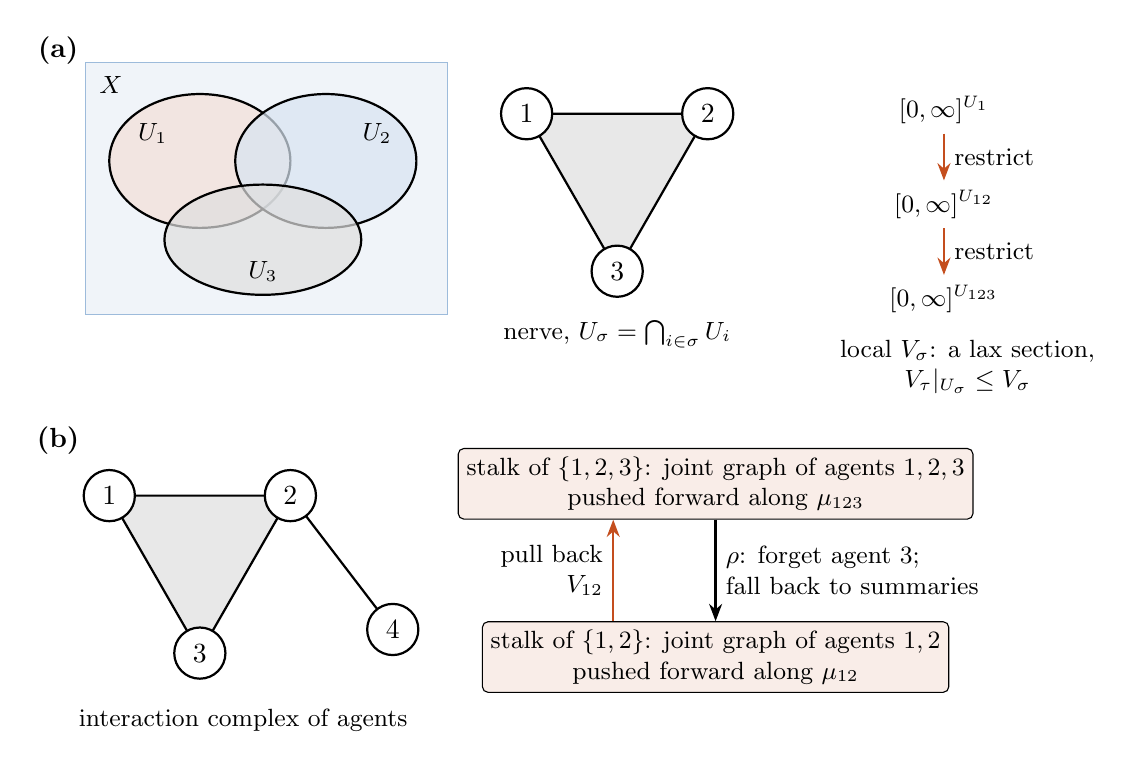
\begin{tikzpicture}[
    lab/.style={font=\small},
    vtx/.style={circle, draw, thick, fill=white, minimum size=6.5mm, inner sep=0pt},
    res/.style={-{Stealth[length=2.2mm]}, thick, accent},
  ]
  % ------------------------------------------------------------ (a) cover and nerve
  \begin{scope}
    \fill[blockfill, draw=blockline] (0,0) rectangle (4.6,3.2);
    \node[lab, anchor=north west] at (0.05,3.15) {$X$};
    \draw[thick, fill=accent!18, fill opacity=0.7] (1.45,1.95) ellipse (1.15 and 0.85);
    \draw[thick, fill=accentB!18, fill opacity=0.7] (3.05,1.95) ellipse (1.15 and 0.85);
    \draw[thick, fill=gray!25, fill opacity=0.7] (2.25,0.95) ellipse (1.25 and 0.7);
    \node[lab] at (0.85,2.3) {$U_1$};
    \node[lab] at (3.7,2.3) {$U_2$};
    \node[lab] at (2.25,0.55) {$U_3$};
    \node[font=\bfseries] at (-0.35,3.35) {(a)};

    % nerve
    \begin{scope}[xshift=5.6cm, yshift=0.35cm]
      \coordinate (n1) at (0,2.2); \coordinate (n2) at (2.3,2.2); \coordinate (n3) at (1.15,0.2);
      \fill[gray!18] (n1) -- (n2) -- (n3) -- cycle;
      \draw[thick] (n1) -- (n2) -- (n3) -- cycle;
      \node[vtx] at (n1) {$1$}; \node[vtx] at (n2) {$2$}; \node[vtx] at (n3) {$3$};
      \node[lab, align=center] at (1.15,-0.6) {nerve, $U_\sigma = \bigcap_{i\in\sigma} U_i$};
    \end{scope}
    % stalks and restrictions
    \begin{scope}[xshift=10.9cm, yshift=0.15cm]
      \node[lab] (F1) at (0,2.45) {$[0,\infty]^{U_1}$};
      \node[lab] (F12) at (0,1.25) {$[0,\infty]^{U_{12}}$};
      \node[lab] (F123) at (0,0.05) {$[0,\infty]^{U_{123}}$};
      \draw[res] (F1) -- node[lab, right, text=black] {restrict} (F12);
      \draw[res] (F12) -- node[lab, right, text=black] {restrict} (F123);
      \node[lab, align=center, anchor=north] at (0.3,-0.35) {local $V_\sigma$: a lax section,\\ $V_\tau|_{U_\sigma} \le V_\sigma$};
    \end{scope}
  \end{scope}

  % ------------------------------------------------------------ (b) agents
  \begin{scope}[yshift=-4.6cm]
    \node[font=\bfseries] at (-0.35,3.0) {(b)};
    \coordinate (a1) at (0.3,2.3); \coordinate (a2) at (2.6,2.3);
    \coordinate (a3) at (1.45,0.3); \coordinate (a4) at (3.9,0.6);
    \fill[gray!18] (a1) -- (a2) -- (a3) -- cycle;
    \draw[thick] (a1) -- (a2) -- (a3) -- cycle;
    \draw[thick] (a2) -- (a4);
    \foreach \i in {1,2,3,4} { \node[vtx] at (a\i) {$\i$}; }
    \node[lab, align=center] at (2.0,-0.55) {interaction complex of agents};

    \begin{scope}[xshift=6.0cm]
      \node[lab, draw, rounded corners=2pt, fill=coarsefill, align=center, inner sep=3pt] (T) at (2.0,2.45)
        {stalk of $\{1,2,3\}$: joint graph of agents $1,2,3$\\ pushed forward along $\mu_{123}$};
      \node[lab, draw, rounded corners=2pt, fill=coarsefill, align=center, inner sep=3pt] (E) at (2.0,0.25)
        {stalk of $\{1,2\}$: joint graph of agents $1,2$\\ pushed forward along $\mu_{12}$};
      \draw[-{Stealth[length=2.2mm]}, thick] (T.south) -- node[lab, right, align=left] {$\rho$: forget agent $3$;\\ fall back to summaries} (E.north);
      \draw[res] ([xshift=-1.3cm]E.north) -- node[lab, left, text=black, align=right] {pull back\\ $V_{12}$} ([xshift=-1.3cm]T.south);
    \end{scope}
  \end{scope}
\end{tikzpicture}

\caption{Sheaves on nerves. (a) A cover $\{U_1,U_2,U_3\}$ of the state space and
its nerve. The canonical sheaf has the value functions on $U_\sigma$ as stalks and
restriction along inclusions as restriction maps. The local cost-to-go functions
form a lax section. (b) For several agents, the cover is of the set of agents (the
clique complex of the interaction graph). Stalks are joint state graphs pushed
forward along symmetric summaries. The restriction $\rho$ forgets an agent and
returns agents out of contact to their summaries. Pulling back a face's cost-to-go
gives a lower bound on the simplex.}
\label{fig:nerve}
\end{figure}

\paragraph{Base change.}
Two commutation facts make these sheaves computable.
\begin{itemize}
\item \emph{Restriction to unions of blocks.} For $U \subseteq Y$ the quotient of
  the subgraph on $\psi^{-1}(U)$ is the restriction of $W_\psi$ to $U$: the minimum
  defining $W_\psi(B,C)$ only involves states of $B$ and $C$. A corridor made of
  whole blocks therefore carries an admissible coarse bound computed from the
  global quotient.
\item \emph{Products.} For two agents moving simultaneously the joint arc cost is
  $W_1(x_1,y_1) + W_2(x_2,y_2)$, where each $W_i$ includes the cost of staying
  put. For a product of abstractions,
  $(W_1 \boxtimes W_2)_{\psi_1 \times \psi_2} = (W_1)_{\psi_1} \boxtimes (W_2)_{\psi_2}$,
  provided each factor's quotient keeps its cheapest move inside a block as a loop.
  The minimum of a sum over a product of blocks is the sum of the minima.
\end{itemize}

\paragraph{Multi-agent covers.}
For $N$ agents, cover the \emph{set of agents} by the clique complex of an
interaction graph, whose edges are the pairs that can meet. The simplices and
their stalks are:
\begin{itemize}[nosep]
\item a simplex $\sigma$ is a set of mutually interacting agents;
\item its stalk is built from the joint state graph of the agents in $\sigma$,
  with collisions removed, pushed forward along a summary map $\mu_\sigma$;
\item $\mu_\sigma$ keeps an agent's exact state when its summary is in contact
  with another agent's summary, and summarizes it otherwise.
\end{itemize}
The restriction to a face forgets the other agents. An agent that was exact only
because of a contact outside the face falls back to its summary. The square
$\rho_{\sigma\tau} \circ \mu_\sigma = \mu_\tau \circ \mathrm{forget}$ commutes, and
$\rho_{\sigma\tau}$ does not increase arc costs. So the pulled-back value of a face
is a lower bound on the simplex.

A joint plan restricts to a plan of every simplex. The per-agent delays $x_a$
(costs in the gauge of the single-agent distances) therefore satisfy
$\sum_{a \in \sigma} x_a \ge \Delta_\sigma$ for the optimal delay $\Delta_\sigma$
of each stalk. The least such integer $0$-cochain bounds the total delay. With
edges alone it is the weighted dependency-graph heuristic of conflict-based
search~\cite{li2019}, whose pair costs are solved exactly there and are
pushforwards here.

\section{Experiments}\label{sec:experiments}

All results come from scripts in \texttt{CellularSheaves.jl/docs/scripts}. The data
are in \texttt{docs/figures}. Each table names its source.

\subsection{A double integrator on a lattice}
The state space has $128^2$ positions times $13^2$ velocities, 2{,}768{,}896 states
in all. One step changes each velocity component by at most one, at unit cost.
Two walls with gaps force the routes to snake. We report means over 30 random
queries (\texttt{tropical\_layered\_study.jl}, \texttt{tropical\_layered.txt}).

The abstraction maps positions and velocities to cells and \emph{velocity modes}
(heading $\times$ speed bins). With one mode it forgets velocity. Forgetting
velocity has large lifting defects. A coarse arc $q \to q'$ costs one step,
because some velocity state moves from $q$ to $q'$ at once. A state in $q$ moving
away from $q'$ at speed $s$ must first brake, which takes about $s$ steps, so the
defect grows with speed. Modes group states whose velocities can follow the same
coarse arcs, which reduces the defect.
\Cref{fig:velocity} shows this on a one-dimensional lattice.

\begin{figure}[t]
\centering
% Forgetting velocity on a one-dimensional lattice double integrator:
% state (p, v) with |v| <= 2, one step chooses v' with |v' - v| <= 1 and sets p' = p + v', cost 1.
% Blocks are the columns (cells). The coarse arc q -> q+1 costs 1; the defect of a state of column q
% is d((q,v), q+1) - 1: 0 for v >= 0, 1 for v = -1, 3 for v = -2.
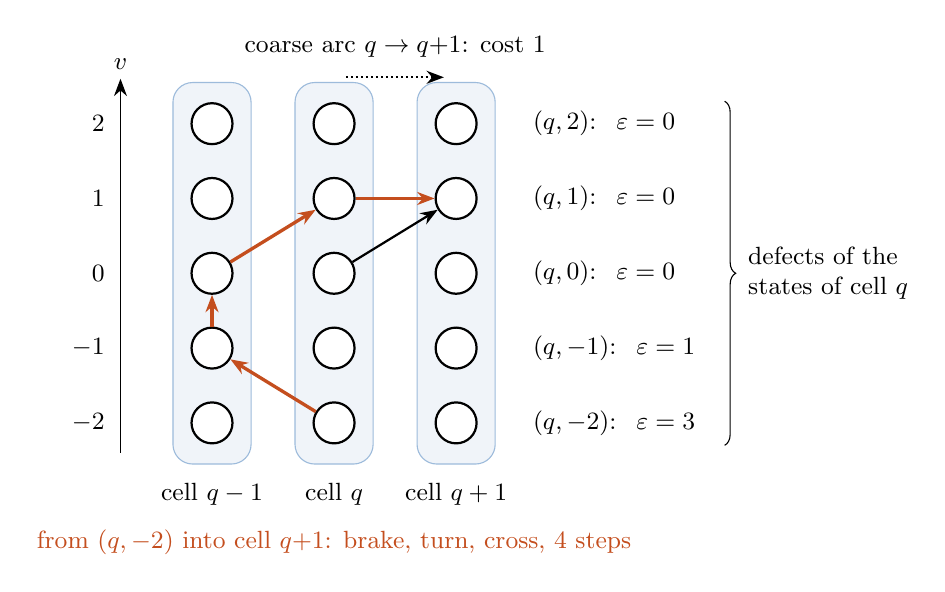
\begin{tikzpicture}[
    x=1.55cm, y=0.95cm,
    st/.style={circle, draw, thick, minimum size=5.2mm, inner sep=0pt, fill=white},
    arc/.style={-{Stealth[length=2.2mm]}, thick},
    path/.style={-{Stealth[length=2.2mm]}, very thick, accent},
    lab/.style={font=\small},
  ]
  % columns q-1, q, q+1 as blocks
  \foreach \c/\name in {0/{q-1}, 1/q, 2/{q+1}} {
    \fill[blockfill, draw=blockline, rounded corners=2.5mm] (\c-0.32,-2.55) rectangle (\c+0.32,2.55);
    \node[lab] at (\c,-2.95) {cell $\name$};
  }
  \foreach \c in {0,1,2} \foreach \v in {-2,...,2} { \node[st] (s\c\v) at (\c,\v) {}; }
  % velocity axis
  \draw[-{Stealth[length=2.2mm]}] (-0.75,-2.4) -- (-0.75,2.6) node[above, lab] {$v$};
  \foreach \v in {-2,...,2} { \node[lab, anchor=east] at (-0.8,\v) {$\v$}; }
  % the coarse arc, realised from (q, 0)
  \draw[arc] (s10) -- (s21);
  \node[lab, anchor=south] at (1.5,2.75) {coarse arc $q \to q{+}1$: cost $1$};
  \draw[arc, densely dotted] (1.1,2.62) -- (1.9,2.62);
  % the optimal way from (q, -2) into cell q+1: brake, turn, cross (4 steps)
  \draw[path] (s1-2) -- (s0-1);
  \draw[path] (s0-1) -- (s00);
  \draw[path] (s00) -- (s11);
  \draw[path] (s11) -- (s21);
  \node[lab, text=accent, anchor=north] at (1.0,-3.3) {from $(q,-2)$ into cell $q{+}1$: brake, turn, cross, $4$ steps};
  % defects of column q
  \foreach \v/\e in {2/0, 1/0, 0/0, -1/1, -2/3} {
    \node[lab, anchor=west] at (2.55,\v) {$(q, \v)$: \ $\eps = \e$};
  }
  \draw[decorate, decoration={brace, amplitude=4pt}] (4.2,2.3) -- (4.2,-2.3)
    node[midway, right=5pt, lab, align=left] {defects of the\\ states of cell $q$};
\end{tikzpicture}

\caption{Forgetting velocity on a one-dimensional lattice double integrator:
$|v| \le 2$, and each unit-cost step chooses $v'$ with $|v' - v| \le 1$ and sets
$p' = p + v'$. The blocks are cells (columns). The coarse arc $q \to q+1$ costs
$1$. From $(q,-2)$, reaching cell $q+1$ takes $4$ steps: brake, turn, cross. The
defect is therefore $3$, and it grows with speed away from the arc's direction.
Velocity modes separate states with different defects.}
\label{fig:velocity}
\end{figure}

\begin{center}
\begin{tabular}{lrrrr}
\toprule
abstraction & coarse states & bound/cost at goal & A$^*$ expansions & time/query \\
\midrule
none (Dijkstra) & -- & -- & 1{,}188{,}243 & 0.245 s \\
forget velocity (1 mode) & 16{,}384 & 0.59 & 142{,}415 & 0.052 s \\
8 headings $\times$ 3 speeds (25 modes) & 409{,}600 & 0.74 & 44{,}188 & 0.022 s \\
16 headings $\times$ 3 speeds (49 modes) & 802{,}816 & 0.79 & 39{,}233 & 0.021 s \\
\bottomrule
\end{tabular}
\end{center}

\paragraph{Corridors (the inclusion as a restriction map).}
A layered controller, in the sense of the layered architectures of Matni, Ames and
Doyle~\cite{matni2024}, plans a route on the abstraction. It then searches the
fine graph exactly, but only inside the pullback of a corridor of cells (and
modes) around the route. The corridor is a union of blocks, so the coarse bound stays
admissible inside it (base change). Restriction to the corridor is the inclusion
restriction of \cref{sec:sheaves}, and its loss is the failure of optimal paths to
stay inside. With corridor width 4:
\begin{itemize}[nosep]
\item forgetting velocity finds a path on the first try for 57\% of queries, at
  1.062 times the optimum on average and 1.545 in the worst case;
\item with 49 modes (mode width 1), 63\%, at 1.006 on average and 1.087 in the
  worst case;
\item at width 16 with 49 modes, every query is optimal.
\end{itemize}

Each closed loop also comes with a certificate in the sense of
\cref{sec:lyapunov}. The corridor cost-to-go $V_U$ is a supersolution of the
whole problem. With the feedback of its shortest-path tree it is checked per
query to be positive, decrescent and strictly decreasing on a closed domain, and
every query was certified. At the query state $x_0$, the closed loop costs
$V_U(x_0)$ (\cref{prop:clf}(iv)). The coarse lower bound gives $V(x_0) \ge
L(x_0)$, so the ratio $V_U(x_0)/L(x_0)$ bounds the suboptimality without knowing
the optimum. It is the pointwise form of the class-$\mathcal K$ gain:
\begin{itemize}[nosep]
\item forgetting velocity: 2.18 on average, 7.50 at worst;
\item 49 modes: 1.30 on average, 1.79 at worst;
\item the true ratios are 1.062 and 1.006.
\end{itemize}

The pessimistic certificate of \cref{thm:lyap-abstraction}(a) is much more
conservative (\texttt{tropical\_lyapunov\_study.jl}). Every state of a mode must
follow the coarse arc in one step, and wide speed bins rarely allow that. It
certifies:
\begin{itemize}[nosep]
\item none of the 2.4 million reachable states with one mode;
\item 9 states with 25 or 49 heading-major modes;
\item 59\% with 8 headings $\times$ 6 speeds, at 2.74 times the optimum on
  average (6.17 at worst);
\item all of them only with one mode per velocity (169 modes).
\end{itemize}
The lifted certificate of \cref{thm:lyap-abstraction}(b) relaxes exactly the
one-step requirement. It has not yet been measured.

\subsection{Cooperative multi-agent planning}
One planner controls all agents, and each agent pays for its steps until it rests
at its goal. In the gauge of the single-agent distances, a heuristic only has to
bound the total \emph{delay}. ``Recovered'' is the share of the coordination cost
(exact joint cost minus the sum of solo distances) that a heuristic's bound closes
at the start, averaged over queries where the agents must cross. All heuristics are
admissible and all searches return the optimum.

\paragraph{Two grid agents.}
The map is $32^2$, with a wall and two one-cell corridors; there are 712{,}336
joint states (\texttt{tropical\_multiagent\_study.jl}). Agent $i$'s abstraction
keeps its own state and summarizes agent $j$:

\begin{center}
\begin{tabular}{lrrr}
\toprule
summary of the other agent & coarse states & recovered & joint A$^*$ expansions \\
\midrule
none (sum of solo distances) & -- & 0\% & 1243 \\
position blocks $4\times 4$ + near field & 62{,}000 & 0\% & 1237 \\
level sets of $\dd_j$ + near field & 105{,}258 & 0\% & 1237 \\
Reeb arcs of $\dd_j$ & 172{,}979 & 89\% & 398 \\
exact joint cost-to-go & 711{,}492 & 100\% & 380 \\
\bottomrule
\end{tabular}
\end{center}

In lifting terms the three summaries fail or succeed for different reasons:
\begin{itemize}[nosep]
\item \emph{Position blocks} forget where in the block $j$ is. A coarse step can
  start from any state of the fibre, so $j$ reaches a corridor ``early'': the
  coarse arc does not lift from $j$'s actual state.
\item \emph{Level sets} of $j$'s cost-to-go fix the timing. But a level set
  contains cells on both sides of the wall, and a coarse arc that leaves the level
  set on one side does not lift from the other.
\item \emph{Reeb arcs} are the connected components of the bands between
  consecutive levels. They separate the two sides~\cite{reeb1946,desilva2016}.
\end{itemize}

\begin{figure}[t]
\centering
% A band of agent j's cost-to-go on a map with a wall: one level set, two Reeb arcs.
% Cells are generated by figures/make_reeb_figure.jl (breadth-first distances).
\begin{tikzpicture}[
    x=4.2mm, y=4.2mm,
    cellfree/.style={fill=white, draw=gray!35, line width=0.2pt},
    arcA/.style={fill=accent!55, draw=gray!35, line width=0.2pt},
    arcB/.style={fill=accentB!55, draw=gray!35, line width=0.2pt},
    wall/.style={fill=black!75, draw=black!75},
    goal/.style={star, star points=5, fill=black, minimum size=3.2mm, inner sep=0pt},
    lab/.style={font=\small},
  ]
  \input{figures/reeb_cells.tex}
  \draw[thick] (0,0) rectangle (17,9);
  \node[lab, anchor=west] at (17.4,7.2) {\textcolor{accent!80!black}{$\blacksquare$}\ Reeb arc $a$};
  \node[lab, anchor=west] at (17.4,6.0) {\textcolor{accentB!80!black}{$\blacksquare$}\ Reeb arc $b$};
  \node[lab, anchor=west, align=left] at (17.4,3.6) {one level set\\ $14 \le \dd_j \le 16$};
  \node[lab, anchor=west] at (17.4,1.0) {$\bigstar$\ goal of $j$};
\end{tikzpicture}

\caption{Level sets versus Reeb arcs. Agent $j$'s goal lies below a wall with
gaps at both ends. Cells are coloured by the band $14 \le \dd_j \le 16$ of its
cost-to-go, computed by breadth-first search
(\texttt{figures/make\_reeb\_figure.jl}). The band is one level set but has two
connected components, the Reeb arcs $a$ and $b$. A summary by level sets puts both
arms in one fibre, so a coarse move available on one side does not lift from the
other. Reeb arcs keep them apart.}
\label{fig:reeb}
\end{figure}

\paragraph{Two double integrators.}
The map is $16^2$ with velocities in $\{-1,0,1\}^2$: 2052 states per agent and
4.2 million pair states
(\texttt{tropical\_multiagent\_double\_integrator.jl}). The near field keeps the
other agent's velocity exactly, or as a mode:

\begin{center}
\begin{tabular}{lrrr}
\toprule
near field keeps & coarse states & recovered & pair A$^*$ expansions \\
\midrule
nothing (decoupled) & -- & 0\% & 1289 \\
rest / moving (2 modes) & 1{,}218{,}918 & 33\% & 994 \\
rest + 4 headings (5 modes) & 1{,}540{,}542 & 67\% & 720 \\
exact velocity (9) & 1{,}969{,}374 & 100\% & 571 \\
exact pair delay & 4{,}192{,}236 & 100\% & 571 \\
\bottomrule
\end{tabular}
\end{center}

\paragraph{The simplicial cover: summaries refined by their futures.}
This study has four to eight agents on a $20^2$ map with two corridors, in 12
instances (\texttt{tropical\_cover\_triangles.jl}, triangle contact radius one
block). It compares two summaries:
\begin{itemize}[nosep]
\item the plain summary (Reeb arc, block);
\item the same summary refined so that the states of a fibre agree on which Reeb
  arcs they can reach along zero-delay moves (\texttt{future\_refinement}).
\end{itemize}
A summarized agent can otherwise ``slide'' along a level set onto another route
for free. That is a coarse walk that does not lift. The full stable refinement of
Paige and Tarjan removes the slide but splits the summaries down to single cells.
The future refinement asks for lifting only at the level of Reeb arcs:

\begin{center}
\begin{tabular}{lcc}
\toprule
& plain summary & future-refined \\
\midrule
edge stalks equal to the exact pair delay & 171 of 175 & 174 of 175 \\
three-agent interactions seen by triangles & 9 of 14 & 13 of 14 \\
coordination cost recovered, $N = 4$ / $N = 6$ & 60\% / 89\% & 100\% / 100\% \\
\bottomrule
\end{tabular}
\end{center}

At $N = 8$ no joint search finishes. The sandwich of the cover bound and a
prioritized plan still certifies the plan within a few percent of optimal.

\paragraph{What we have not yet measured.}
The experiments above predate the theorem. We read them through it, but we have
not yet computed the defects themselves. Computing the defects of each map, and
correlating them with the measured bounds, is the next step (issue~019 in the
repository).

\section{Related work}

\paragraph{Path algebra.}
Shortest paths, bottleneck paths and transitive closure are one problem over
closed semirings, solvable by elimination~\cite{carre1971,lehmann1977,tarjan1981,
gondran2008}. Residuation in idempotent semimodules supplies the Galois
connections we use~\cite{baccelli1992,cohen2004}.

\paragraph{Abstraction and aggregation.}
\begin{itemize}[nosep]
\item Aggregation in dynamic programming~\cite{bertsekas1989} and multigrid for
  stochastic control~\cite{chow1991} work in the real semiring, where coarse
  solutions correct rather than bound.
\item Abstraction heuristics include Hierarchical A$^*$~\cite{holte1996},
  pattern databases~\cite{culberson1998} and merge-and-shrink~\cite{helmert2007}.
\item Abstraction-based control relies on refinement relations between a system
  and its abstraction~\cite{tabuada2009,reissig2017}.
\end{itemize}
The lifting defect is a quantitative, cost-aware version of the conditions under
which an abstraction is exact.

\paragraph{Sheaves and lattices.}
Cellular sheaves and their Laplacians~\cite{curry2014,hansen2019} have lattice-valued
analogues: the Tarski Laplacian~\cite{ghrist2022} and its quantale-enriched
generalization, the Lawvere Laplacian~\cite{ghrist2025diffusion}. Reeb graphs are
cosheaves~\cite{desilva2016}.

\paragraph{Lyapunov theory.}
Categorical Lyapunov theory~\cite{ames2025clt1,ames2025clt2} supplies the notion
of Lyapunov morphism we use. Our contributions there are the identification of
the norm with the cost-to-go, certified class-$\mathcal K$ gains, and certificates
transported from abstractions. Layered planning and control architectures are
surveyed by Matni, Ames and Doyle~\cite{matni2024}.

\paragraph{Multi-agent path finding.}
Our cover bound with edges alone is the weighted dependency-graph heuristic of
conflict-based search~\cite{sharon2015,li2019}. Independence detection merges
agents only when their plans collide~\cite{standley2010}.

\section{Limitations and open problems}
\begin{itemize}
\item The theorem is for deterministic, finite problems. Stochastic aggregation
  belongs to the real semiring.
\item The space--time abstractions of our studies (coarse arcs that are $k$-step
  moves) are not covered as stated.
\item The quantitative bound charges the largest defect on every arc of a walk. A
  per-arc bound is available (\cref{thm:sandwich}), but choosing abstractions to
  minimize it is open. The defect is a natural refinement signal, as in
  counterexample-guided abstraction refinement.
\item The lax functor of fibres is stated over the indiscrete category on blocks. A
  statement over the path category of the quotient, in the generality of
  Bénabou's correspondence, would make the fibre picture functorial in the
  abstraction.
\end{itemize}

\bibliographystyle{plain}
\bibliography{references}

\end{document}
